\chapter{Electrochemical Energy Storage in Redox Conductive Polymers}

\section{Rechargeable Electrochemical Cells}

The capacity of installed battery storage systems is predicted to increase upto 400~GWh by 2030~\cite{Figgener_2020}.

State of charge (SoC).\\
State of health (SoH).\\
Gravimetric capacity.\\




\section{Redox Conductive Polymers}

Redox active macromolecules or polymers~\cite{Staudinger_1920} are known since 1940s due to the works of Lauth~\cite{Lauth_1944} and Cassidy~\cite{Cassidy_1949} on electron exchange polymers. After the discovery of the conductivity of polyacetylene by Shirakawa, Heeger and McDiarmid in 1977~\cite{Shirakawa_1977}, polymers with sufficient charge transport were synthesized~\cite{} and the field of organic electronics had emerged and expanded. 

\par

The key for polymer conductivity is the p $\pi$ - conjugated network, a system of overlapping $\pi$ orbitals of carbon in a chain of alternating single and double carbon-carbon bonds that allows charge delocalization along the polymer backbone. An example of a $\pi$ conjugated network is polyacetylene. Polyacetylene exhibits a band structure in the electron energy levels (between $\pi$ and $\pi^\star$ orbitals) and represents a molecular semiconductor.

\par

Organic solar cells~\cite{Lee_1993} and organic field effect transistors~\cite{Koezuka_1987} contain conjugated polymers that have electrical properties of semiconductors, yet can be easily printed in form of thin flexible films without using high temperatures. Combining the conductive polymers with stable radical side groups has formed the class of redox conductive polymers and lead to the concept of an organic radical battery~\cite{Rohland_2021}.




\section{Organic Radical Battery}

Batteries based on conjugated polymers containing stable radical moieties as high-capacitance groups represent a promising class of future electrochemical power sources - organic radical batteries (ORB)~\cite{nakahara2002_cpl, nishide2004_electact,xie2021_mathoriz,Rohland2022}. ORB combine the advantages of high-power supercapacitors, namely high discharge rates, and the high energy density of conventional lithium-ion technology. In contrast to the lithium-ion battery, the charging of an organic battery does not involve intercalation of metal ions into the electrodes. This reduces the structural change of the electrode upon repeated recharging which allows for a longer cycle life of an ORB. The semi-conducting nature of organic electrodes reduces the Joule heating during the battery operation, and this allows for higher charge/discharge rates. The amorphous and swollen structure of organic electrodes allows the electrolyte ions to diffuse faster into the electrode, which also increases the charge/discharge rate~\cite{nishide_2009}. A further beneficial property of organic materials over traditional inorganic materials is their availability and the low cost of the starting materials for the synthesis of the target polymers in conjunction with good mechanical properties~\cite{janoschka2012_advmater, muench2016_chemrev, friebe2017_topcurrchem}. The large knowledge base on polymer processing allows for inkjet printing, roll-to-roll processing and other low-cost manufacturing techniques for making low-cost, flexible and light-weight integrated devices, including flexible plastic batteries~\cite{janoschka2012_advmater,nishide_2009}. 
\par


\section{Organic Electrode Materials}
ORB based on redox polymers containing stable radicals~\cite{nakahara2002_cpl} have been shown to compete with or even outperform  conventional Li based batteries in terms of power densities~\cite{IWASA2007} with the additional benefit of being free from rare precursors, inheriting mechanical properties of plastics and electrical properties of semiconductors~\cite{friebe2017_topcurrchem,Casado2021,Goujon2021}. Advanced molecular design techniques allow for tuning of the electrochemical properties of the redox polymers~\cite{Janoschka2017}, that brings in a rich variety of organic energy storage materials~\cite{Xie2021,Vereshchagin2022,Janoschka2017a} and creates a large room for their optimization. 

\par
\subsection{TEMPO}
TEMPO (2,2,6,6-tetramethylpiperidine-1-oxyl) shown in Figure~\ref{fig:molecules}~a) is a small molecule and a stable radical that can undergo a fast and revirsible redox reaction between TEMPO$^\bullet$ and TEMPO$^+$. TEMPO is an inexpensive organic compound~\cite{Vereshchagin2022} produced from acetone with liquid ammonia, hydrazine and peroxide~\cite{Casado_2021_book}. TEMPO radicals are widely used as spin labels in biological systems.

TEMPOL is a TEMPO with an OH group.

\begin{figure}[h]
\center
	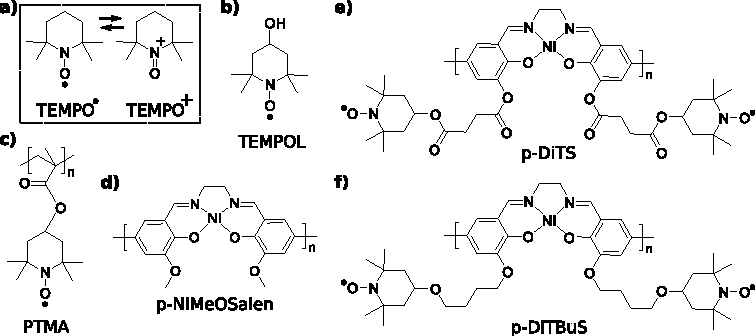
\includegraphics[width=1\textwidth]{./electrochemistry/figures/materials/molecules.pdf}
	\caption{Chemical structures of the molecular fragments that were used for making a battery cathode containing stable nitroxide radicals.}
	\label{fig:molecules}
\end{figure}



Redox conductive conjugated polymers containing TEMPO redox groups, as pDiTBuS (poly-di-TEMPO-Butyl-Salen) shown in Figure~\ref{fig:Figure_1}, demonstrate particularly promising energy and power densities~\cite{Vereshchagin2020}. The pDiTBuS was designed as a cathode material: it is oxidized when the electrochemical cell containing this material is charged. A film of pDiTBuS comprises a high concentration of redox active stable nitroxyl radicals attached to a conjugated polymer backbone that interconnects them as a molecular wire. Such system can be viewed as a highly disordered molecular hole-transporting semiconductor (the poly-NiSalen backbone) that contains a large amount of hole traps (TEMPO groups) attached to it with butyl linkers. When the film is reduced (discharged), the TEMPO groups are in the radical state and act as unfilled traps. Upon oxidation (charging), the TEMPO fragments lose an unpaired electron and acquire a positive charge, so the traps are being filled with holes. The reversible redox reaction in the pDiTBuS film is demonstrated in a cyclic \ik{voltammogram} shown in Figure~\ref{fig:Figure_S1} (see ESI).

\par
While active electrode materials with nitroxide radicals as redox-active groups are ideally suited for organic radical batteries (ORBs) that exhibit high power densities, the broad application of most nitroxide-based materials is limited by their moderate electrical properties. A promising route towards overcoming the conductivity problem is the use of polymers that combine radical-containing moieties and a conductive backbone. This strategy was successfully followed in a number of studies focusing on different polymers.\cite{oyaizu2015_polymerjournal, bahaceci2013_jpowersources, katsumata2006_mrc, xu2014_electact, aydin2015_jsoistatelect, schwartz2018_synthmet}

\par

The flexible molecular design together with questions regarding unresolved charge transport- and performance limiting mechanisms have inspired a variety of characterization techniques to be developed and applied to both energy storage materials and energy storage devices, operando and ex-situ. Together with electrochemical characterization as the standard method for studying the properties of energy storage materials\cite{IWASA2007,Zens2022}, operando optical microscopy~\cite{Merryweather2022}, neutron imaging~\cite{Ma2020} and X-ray diffraction~\cite{Rhodes2012} were applied to monitor irreversible structural deformations during extreme charging of Li cells.

\subsection{PTMA}

A simple organic radical polymer containing TEMPO is poly(2,2,6,6-tetramethyl-1-piperidinyloxy-4-yl methacrylate) (PTMA, Figure~\ref{fig:molecules}~c). The polymer backbone of PTMA consists of single C-C bonds and therefore is not conductive, so the transport of charge in a PTMA film has to be mediated by adding conductive mesh such as activated carbon. When mixed with conductive carbon additive, PTMA has become a standard cathode material for ORBs and Li-ORBs, providing a discharge cell voltage of 3.5~V (with a Li anode) and a theoretical discharge capacity of $C_{theo}=111$~mAh/g~\cite{Daniel2023_Multimodal}. PTMA is soluble in acetonitrile (AN), chloroform (CF), tetrahydrofurane and dichlormethane. It is claimed to be insoluble in toluene, ethers, carbonates, and alcohols, however it becomes gel-like with some of these solvents~\cite{DOM}.

\subsection{NiSalen}



\subsection{pDiTBuS}
Redox conductive conjugated polymers containing TEMPO (2,2,6,6-tetramethylpiperidine-1-oxyl) redox groups, as pDiTBuS (poly-di-TEMPO-Butyl-Salen) shown in Figure~\ref{fig:Figure_1}, demonstrate particularly promising energy and power densities~\cite{Vereshchagin2020}. The pDiTBuS was designed as a cathode material: it is oxidized when the electrochemical cell containing this material is charged. A film of pDiTBuS comprises a high concentration of redox active stable nitroxyl radicals attached to a conjugated polymer backbone that interconnects them as a molecular wire. Such system may be viewed as a highly disordered molecular hole-transporting semiconductor (the poly-NiSalen backbone) that contains a large amount of hole traps (TEMPO groups) attached to it with butyl linkers. When the film is reduced (discharged), the TEMPO groups are in the radical state and act as unfilled traps. Upon oxidation (charging), the TEMPO fragments lose an unpaired electron and acquire a positive charge, so the traps are being filled with holes.

\begin{figure}[h]
\center
	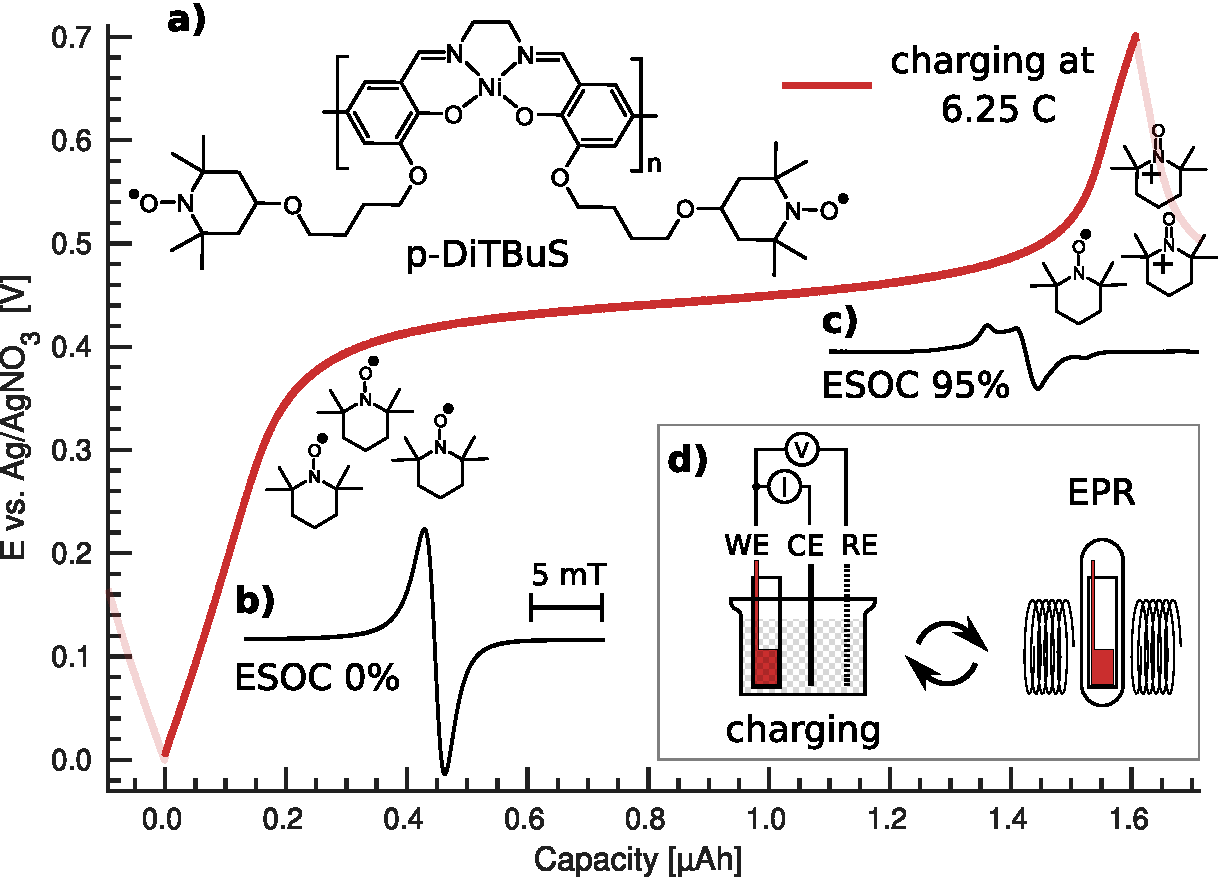
\includegraphics[width=0.7\textwidth]{./introduction/figures/Figure_1.pdf}
	\caption{Galvanostatic charge-discharge curve for a pDiTBuS cathode film at 10~$\muup$A (6.25~C), chemical structure of pDiTBuS (a), normalized cwEPR spectral signatures for reduced (b) and oxidized (c) states. Scheme of the ex-situ EPR measurement on the pDiTBuS half cell (d).}
	\label{fig:Figure_1}
\end{figure}

\subsection{pDiTS}
\subsection{Density Functional Theory Calculation of Spin Density on DiTS}
\begin{figure}[h]
\center
	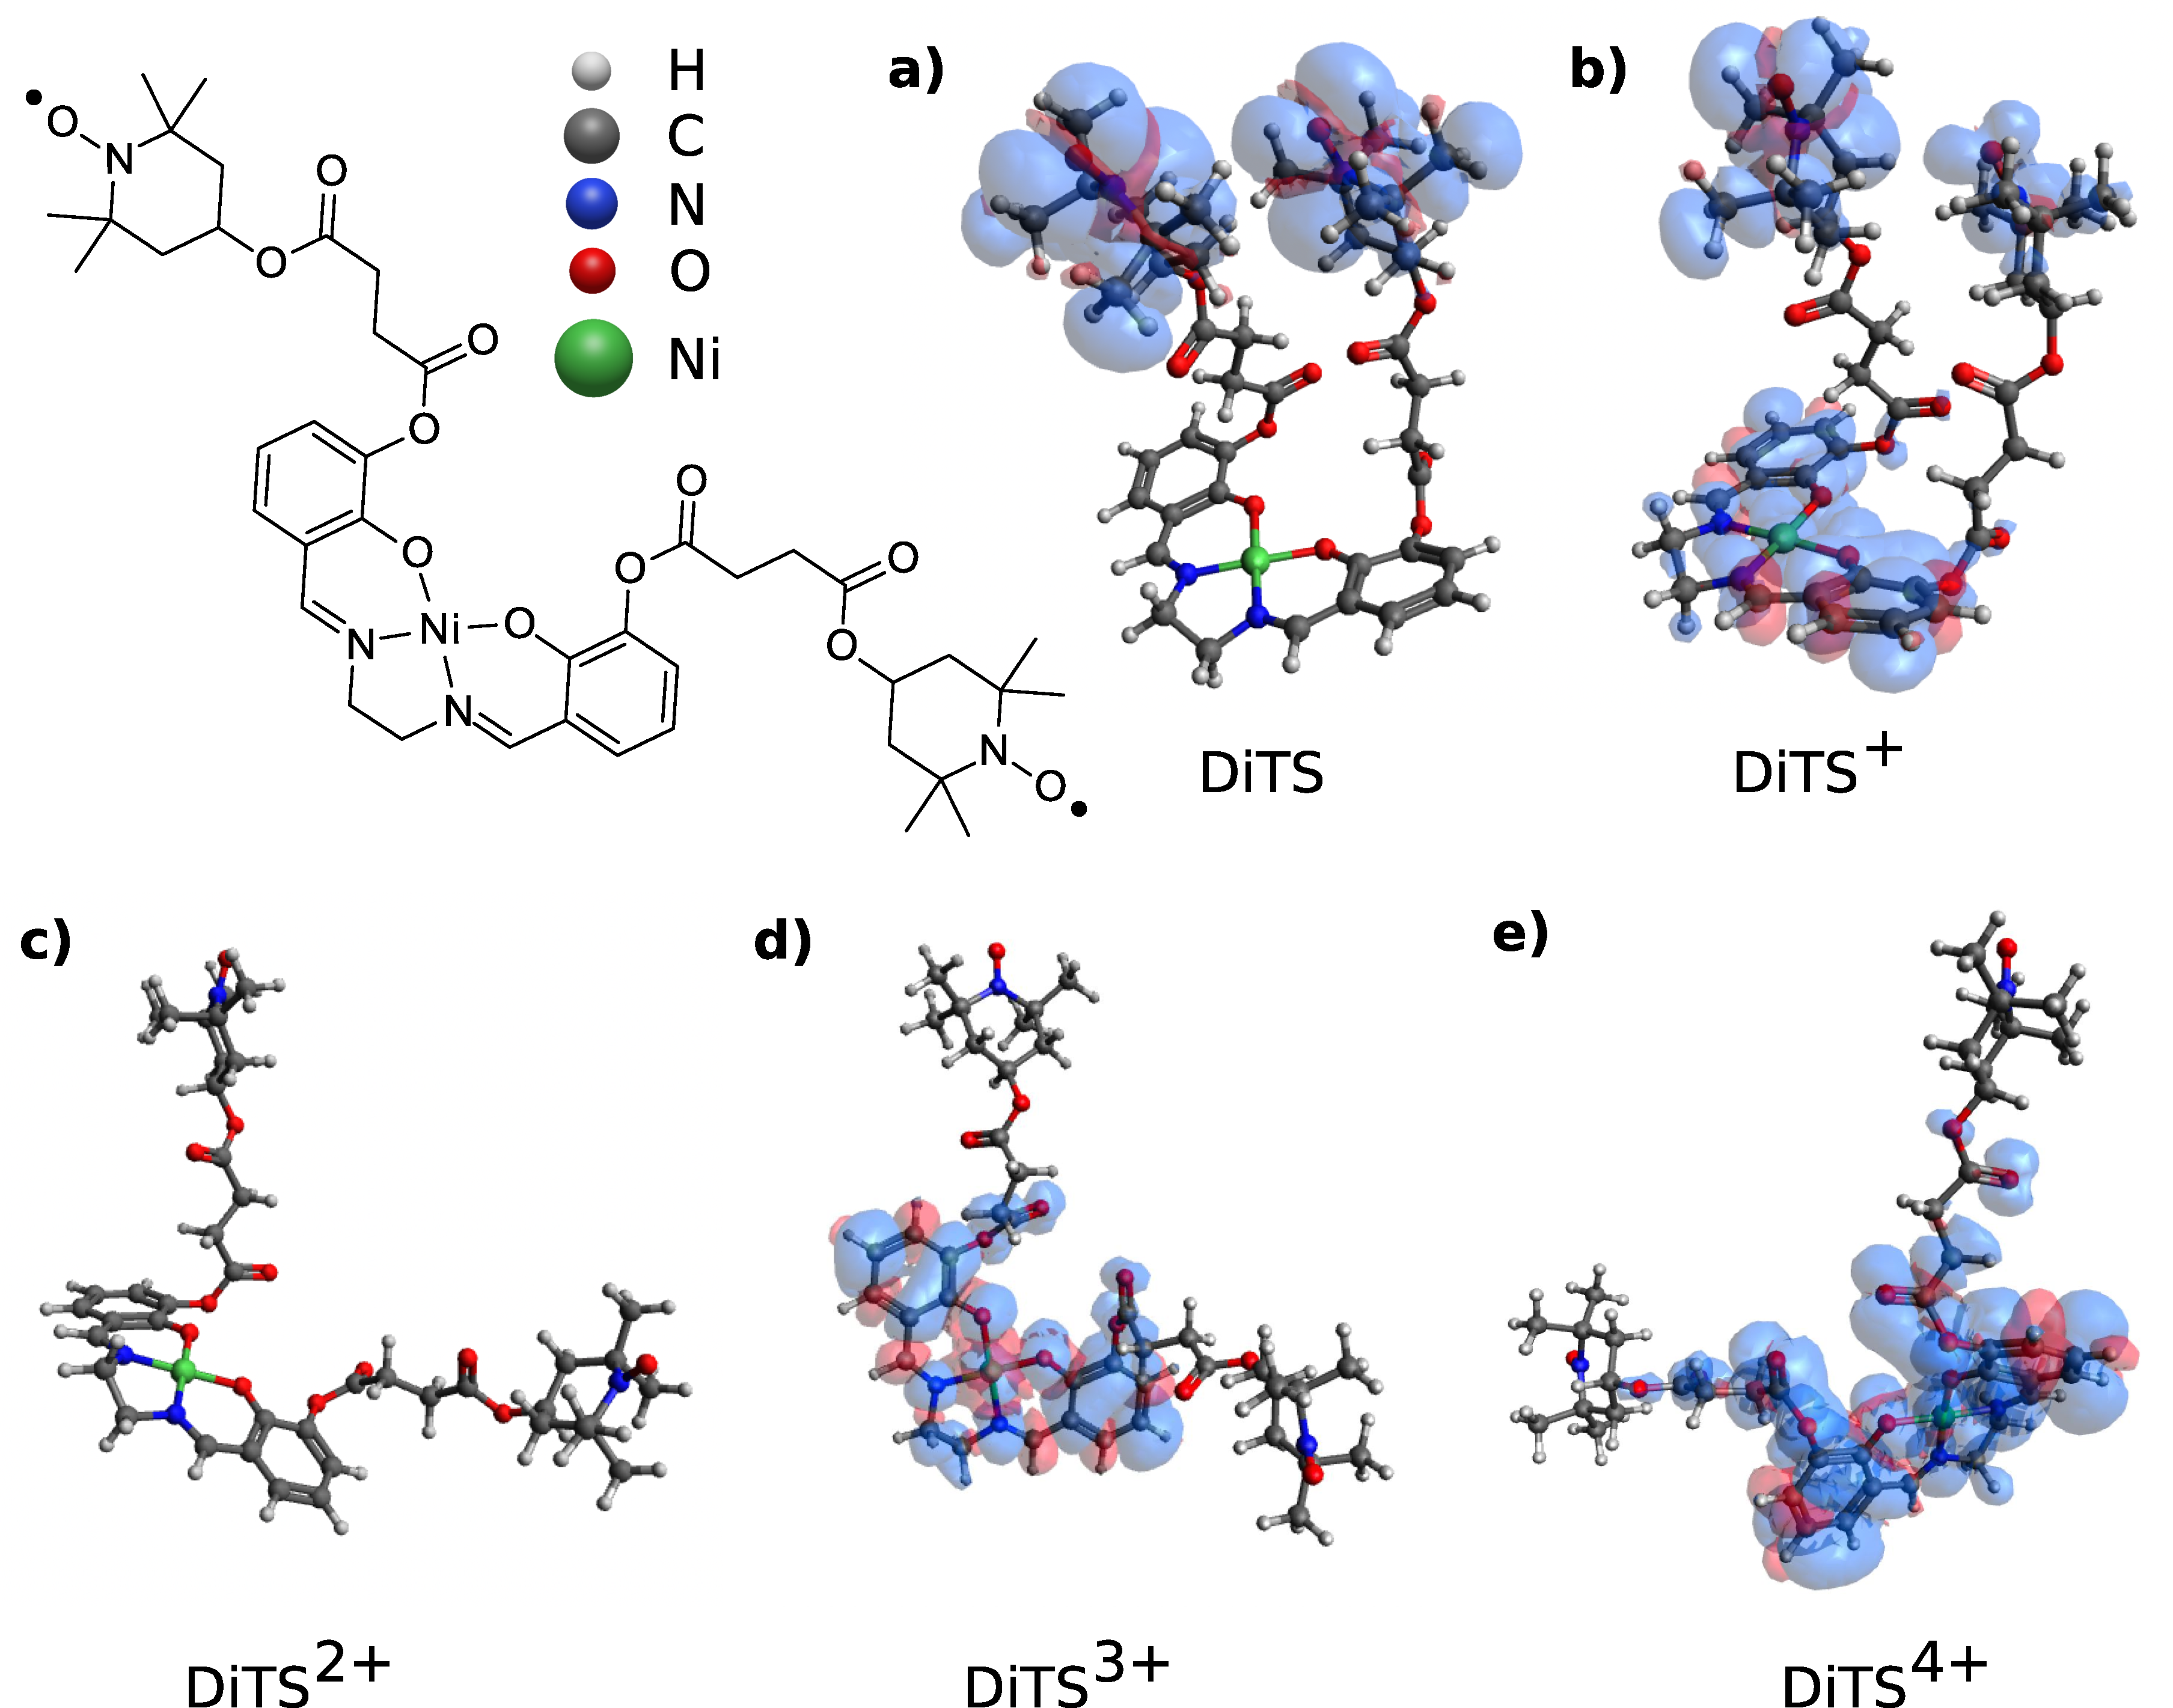
\includegraphics[width=1\textwidth]{./electrochemistry/figures/DFT_DITS.pdf}
	\caption{Spin density in a single DiTS monomer unit for various oxidation states calculated by Marcel Gauglitz with density-functional theory in ORCA~\cite{ORCA} at the high-performance computing cluster of the Free University Berlin~\cite{HPC_FUB} using the def2-TZVP functional basis set. a): neutral DiTS with two radicals, b) singly oxidized DiTS (one hole injected), b) doubly oxidized DiTS showing no spin density, c) DiTS$^{3+}$ showing a positive polaron localized on the NiSalen backbone, d) DiTS$^{4+}$ showing increased spin density on the backbone.}
	\label{fig:DiTS_DFT}
\end{figure}



\subsection{Charge Transport Model for Redox Conductive Polymers}
A transfer of charge in a highly disordered molecular system, such as a film of a conjugated polymer, can be described in terms of hopping of charge carriers between the intertwined polymer fragments under external electric field. The molecular systems for electrochemical charge storage are inherently disordered materials and the electric performance of a film containing those molecules is is strongly dependent on the deposition method, as well as on the molecular structure See \cite{Xie2021} (!). Therefore, so far there has not been a unified physical model that would describe the charge transport phenomena in such materials. The particular charge transport models have been developed that are applicable to certain classes of polymers (read that chapter in the polymer book and show what was done). 




